\documentclass[12pt,a4paper]{article}
\usepackage[utf8]{inputenc}
\usepackage[brazil]{babel}
\usepackage{graphicx}
\usepackage{amssymb, amsfonts, amsmath}
\usepackage{float}
\usepackage{enumerate}
\usepackage[top=2.5cm, bottom=2.5cm, left=1.25cm, right=1.25cm]{geometry}

\begin{document}
\pagestyle{empty}

\begin{center}
  \begin{tabular}{ccc}
    \begin{tabular}{c}
      
\includegraphics[scale=0.25]{../../biblioteca/imagem/brasao-de-armas-brasil} \\
    \end{tabular} & 
    \begin{tabular}{c}
      Ministério da Educação \\
      Universidade Federal dos Vales do Jequitinhonha e Mucuri \\
      Faculdade de Ciências Sociais, Aplicadas e Exatas - FACSAE \\
      Departamento de Ciências Exatas - DCEX \\
      Disciplina: Matemática Elementar I \quad Semestre: 2021/1\\
      Prof. Me. Luiz C. M. de Aquino\\
    \end{tabular} &
    \begin{tabular}{c}
      
\includegraphics[scale=0.25]{../../biblioteca/imagem/logo-ufvjm} \\
    \end{tabular}
  \end{tabular}
\end{center}

\begin{center}
  \textbf{Lista IV}
\end{center}

\begin{enumerate}
  \item Determine a função $f$ polinomial do 1° grau tal que seu gráfico passa
  pelos pontos $(2,\,-4)$ e $(6,\,-2)$.
  
  \item Os gráficos das funções $f$ e $g$ estão ilustrados abaixo. Determine o
  ponto de interseção entre esses gráficos.
  
    \begin{figure}[H]
     \centering
     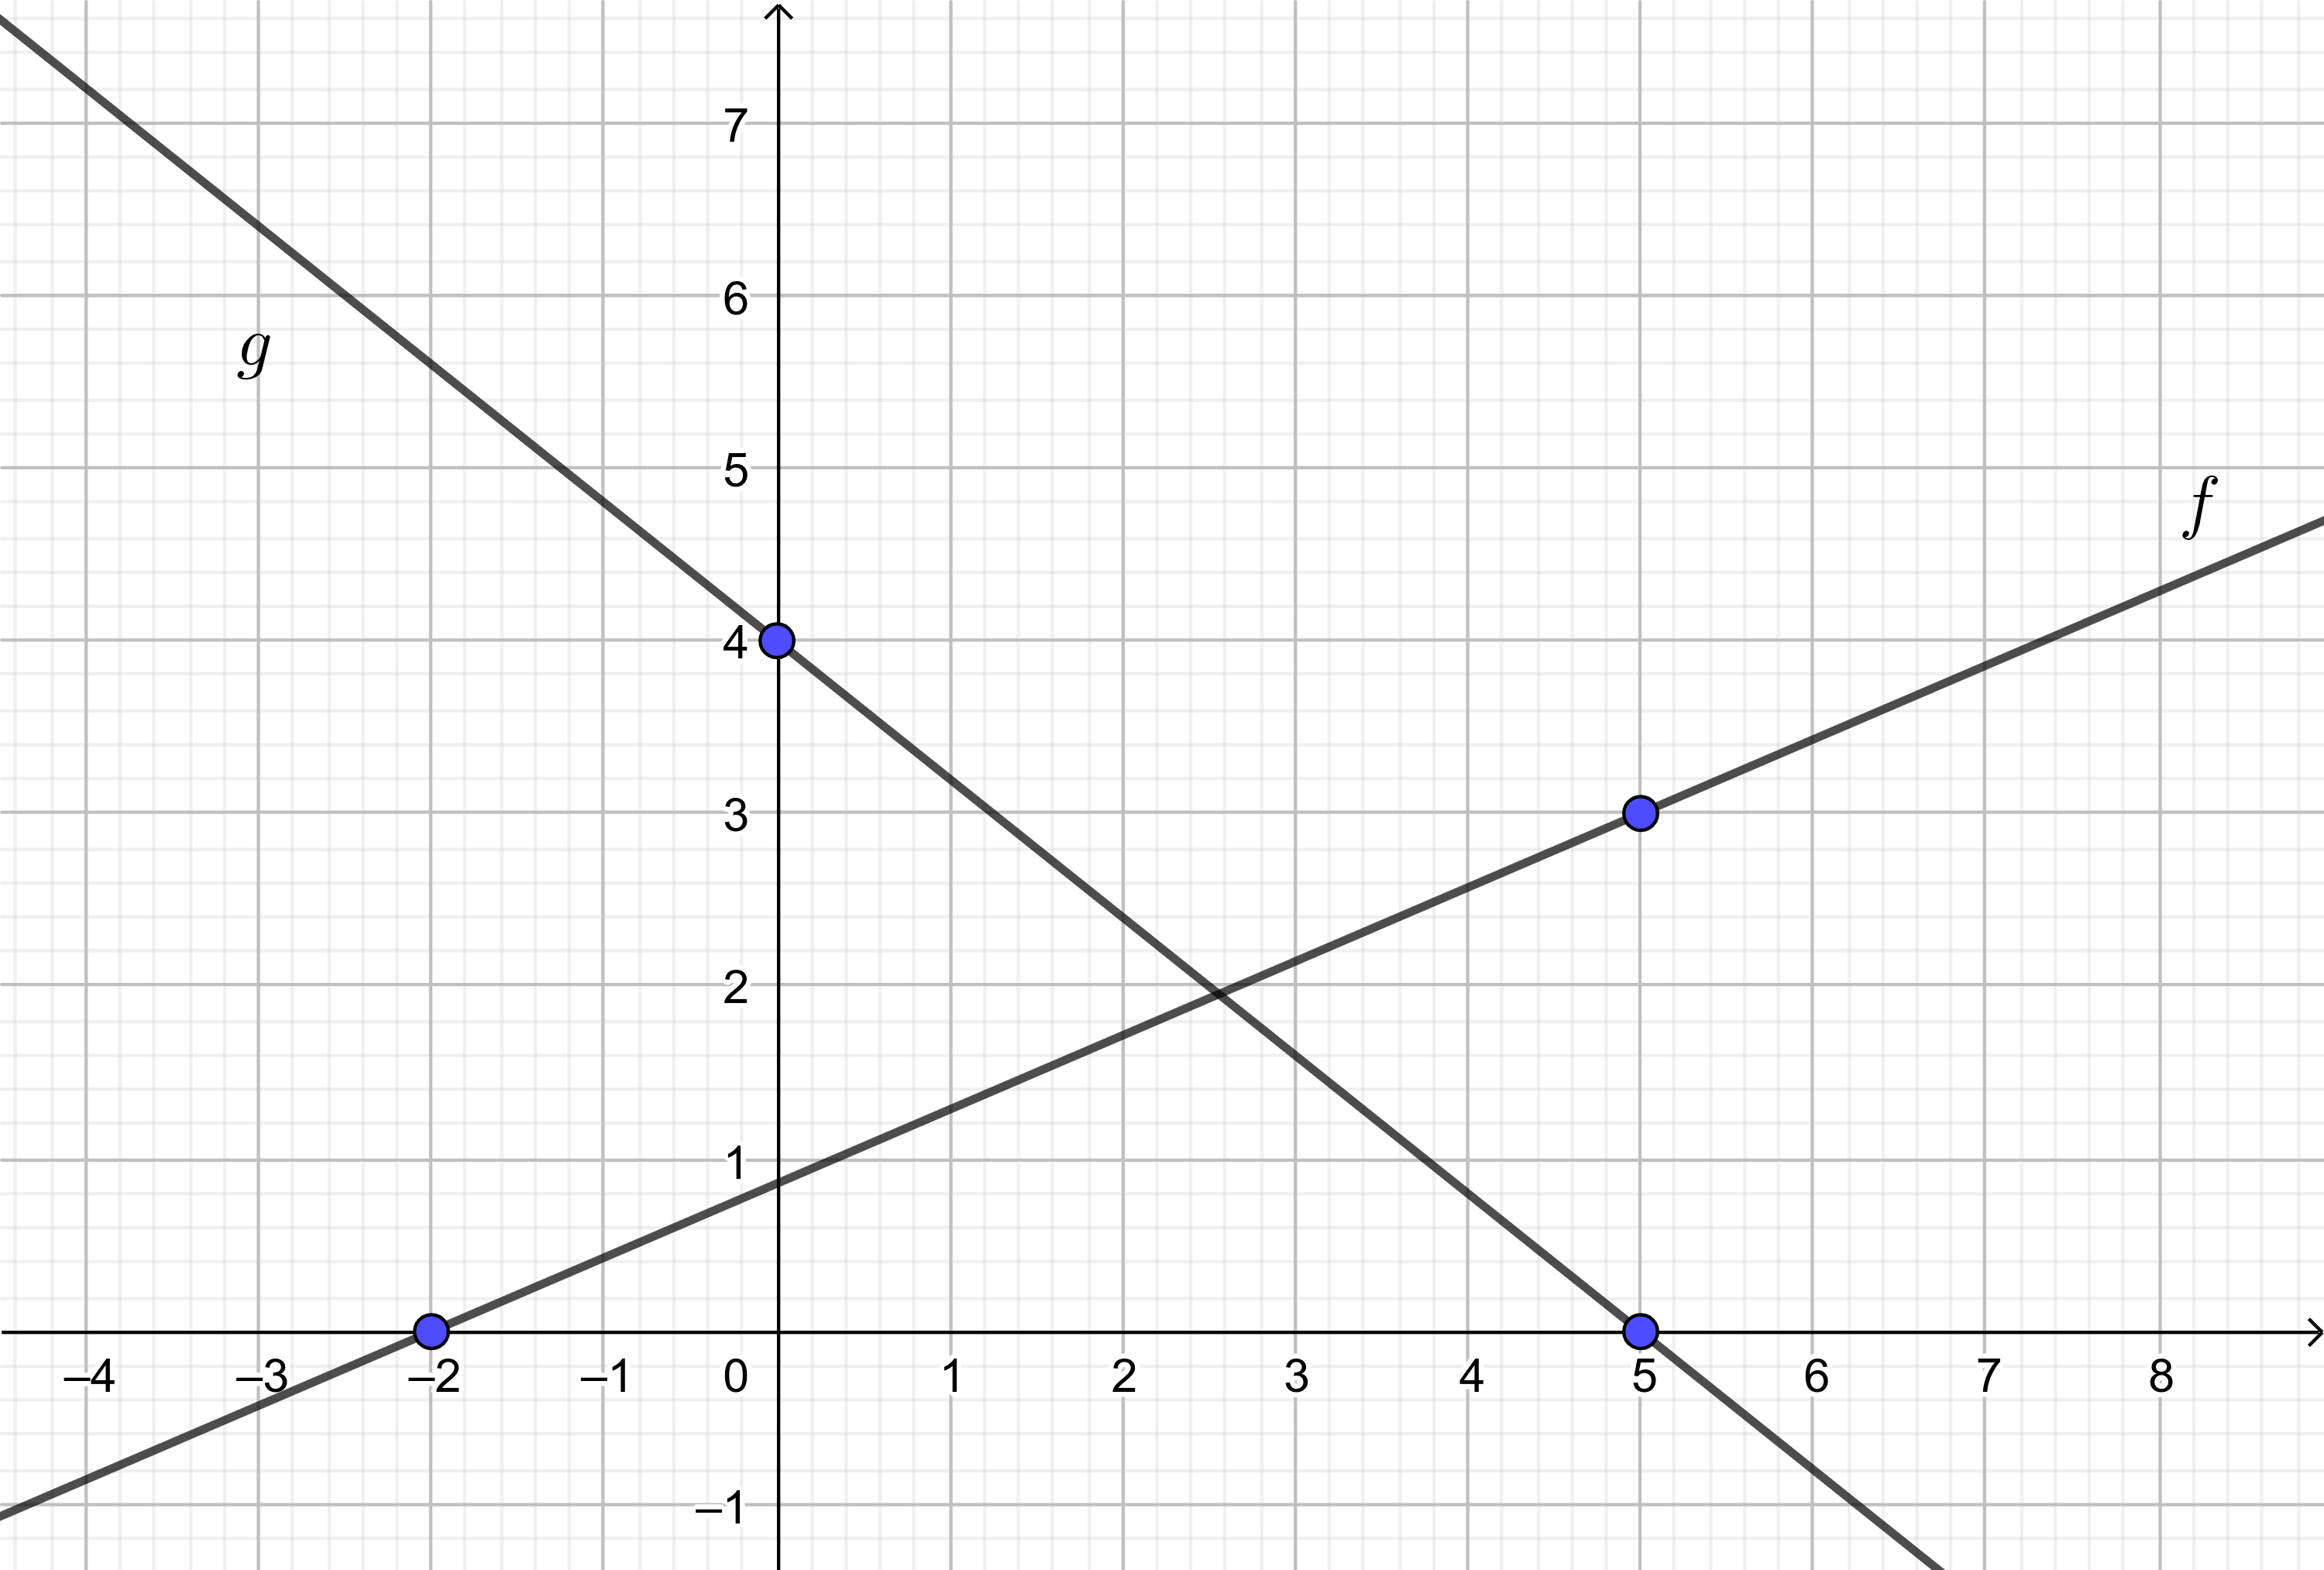
\includegraphics[scale=0.75]{figura/grafico-lista-iv-21-1.png}
    \end{figure}

  \item Determine o domínio das funções definidas abaixo.
  \begin{enumerate}
    \item $f(x) = \dfrac{\sqrt{(x + 1)(10 - 4x)}}{x - 1}$.
    \item $g(x) = \dfrac{\sqrt{x(2 - x)} + \sqrt{(x - 1)(x - 3)}}{x^2 + 4}$.
  \end{enumerate}
  
  \item Em certa loja de calçados os vendedores recebem de salário 
  um valor fixo de R\$ 1.500,00 e mais uma comissão de 2,5\% sobre o total de
  vendas que eles efetuarem no mês. Se em certo mês um vendedor recebeu
  R\$ 1.965,00 de salário, então qual foi o total de vendas dele nesse mês?
  
  \item Suponha que $f$ seja uma função polinomial do 1° grau tal que
  $f(0) = m$ e $f(1) = n$. Prove que $f(x) = m(1 - x) + nx$.

\end{enumerate}

\begin{center}
  \textbf{Gabarito}
\end{center}

[1] $f(x) = \dfrac{1}{2}x - 5$. 
[2] $\left(\dfrac{110}{43},\, \dfrac{84}{43}\right)$. 
[3]
(a) $D = \left\{x\in \mathbb{R}\,|\, -1 \leq x \leq \dfrac{5}{2} \textrm{ e }x \neq 1\right\}$. 
(b) $D = \left\{x\in \mathbb{R}\,|\, 0 \leq x \leq 1\right\}$. 
[4] R\$ 18.600,00. 
[5] Sugestão: considerando que $f(x) = ax + b$, resolva o sistema de equações formado por
$f(0) = m$ e $f(1) = n$. 

\end{document}